\documentclass[a4paper,12pt,oneside,openany]{book}	
\usepackage{layout}
\setlength{\textwidth}{15.0 cm}
\setlength{\textheight}{25.0 cm}


\usepackage[english,brazil]{babel}
\usepackage{pagina}	% pagina-padrao
\usepackage{indentfirst}		% for indent
\usepackage[utf8]{inputenc}
\usepackage{graphics,epsfig}
\usepackage{graphics}
\graphicspath{{./figuras/}}
\usepackage{pstricks,pst-node,pst-tree}
\usepackage{alltt}
%\usepackage{makeidx}
%\makeindex
\usepackage[figuresright]{rotating} % for saydways tables and figures
\usepackage{enumerate}			% for configuration of enumerate environment
\usepackage{amsmath}
\usepackage{amssymb}
\usepackage{portland,multirow}

\setcounter{secnumdepth}{3}	% numeracao ate subsubsecao
\setcounter{tocdepth}{2}	% indice ate subsubsecao

\usepackage{longtable}

% meus pacotes
\usepackage{subcaption}
\usepackage{float}


\begin{document}

\frontmatter
\thispagestyle{empty}


\includegraphics[scale=0.7]{Poli.eps}

\begin{center}
\large{DESENVOLVIMENTO DE BASE DE DADOS PARA TREINAMENTO DE REDES NEURAIS DE RECONHECIMENTO DE VOZ ATRAVÉS DA GERAÇÃO DE ÁUDIOS COM RESPOSTA
AO IMPULSO SIMULADAS POR TÉCNICAS DE DATA AUGMENTATION}\\
   \vspace{2cm}
\large{Bruno Machado Afonso}\\
\end{center}
   \vspace{3cm}
\hspace{7cm}
\hfill \parbox{8.0cm}{Projeto de Graduação apresentado ao Curso de Engenharia Eletrônica e de Computação da Escola Politécnica,
Universidade Federal do Rio de Janeiro, como parte dos requisitos necessários à obtenção do título de Engenheiro.\\}
   \vspace{2cm}
\hfill \parbox{8.0cm}{Orientador: Mariane Rembold Petraglia} \\
   \vspace{2cm}
\begin{center}
Rio de Janeiro

Julho de 2021
\end{center}




\pagebreak


\begin{center}
\large{DESENVOLVIMENTO DE BASE DE DADOS PARA TREINAMENTO DE REDES NEURAIS DE RECONHECIMENTO DE VOZ ATRAVÉS DA GERAÇÃO DE ÁUDIOS COM RESPOSTA
AO IMPULSO SIMULADAS POR TÉCNICAS DE DATA AUGMENTATION}\\
   \vspace{1cm}
\large{Bruno Machado Afonso}\\
\end{center}
   \vspace{2cm}
PROJETO DE GRADUAÇÃO SUBMETIDO AO CORPO DOCENTE DO CURSO DE ENGENHARIA ELETRÔNICA E DE COMPUTAÇÃO DA ESCOLA POLITÉCNICA DA
UNIVERSIDADE FEDERAL DO RIO DE JANEIRO COMO PARTE DOS REQUISITOS NECESSÁRIOS PARA A OBTENÇÃO DO GRAU DE ENGENHEIRO ELETRÔNICO E DE COMPUTAÇÃO   
   
   \vspace{1cm}
Autor:
      \vspace{0.5cm}
      \begin{flushright}
         \parbox{10cm}{
            \hrulefill

            \vspace{-.375cm}
            \centering{Bruno Machado Afonso}

            \vspace{0.1cm}
         }
      \end{flushright}
      
      
Orientador:
      \vspace{0.5cm}
      \begin{flushright}
         \parbox{10cm}{
            \hrulefill

            \vspace{-.375cm}
            \centering{Profª. Mariane Rembold Petraglia, Ph. D.}

            \vspace{0.1cm}
         }
      \end{flushright}
      
Examinador:
      \vspace{0.5cm}
      \begin{flushright}
         \parbox{10cm}{
            \hrulefill

            \vspace{-.375cm}
            \centering{Prof. A SER DEFINIDO, D. Sc.}

            \vspace{0.1cm}
         }
      \end{flushright}
      
Examinador:
      \vspace{0.5cm}
      \begin{flushright}
         \parbox{10cm}{
            \hrulefill

            \vspace{-.375cm}
            \centering{Prof. A SER DEFINIDO, D. E.}

            \vspace{0.1cm}
         }
      \end{flushright}
      
                        
      \vfill
      
      
\begin{center}
Rio de Janeiro

Julho de 2021
\end{center}


\pagebreak            

% Declaracao
\begin{center}
Declaração de Autoria e de Direitos
\end{center}

\vspace{0.4cm}

Eu, \emph{Bruno Machado Afonso} CPF \emph{136.151.347-02}, autor da monografia \emph{Desenvolvimento de Base de Dados para Treinamento de Redes Neurais de Reconhecimento de Voz Através da Geração de Áudios com Resposta
ao Impulso Simuladas por Técnicas de Data Augmentation}, subscrevo para os devidos fins, as seguintes informações:\\
1. O autor declara que o trabalho apresentado na disciplina de Projeto de Graduação da Escola Politécnica da UFRJ é de sua autoria, sendo original em forma e conteúdo.\\
2. Excetuam-se do item 1. eventuais transcrições de texto, figuras, tabelas, conceitos e ideias, que identifiquem claramente a fonte original, explicitando as autorizações obtidas dos respectivos proprietários, quando necessárias.\\
3. O autor permite que a UFRJ, por um prazo indeterminado, efetue em qualquer mídia de divulgação, a publicação do trabalho acadêmico em sua totalidade, ou em parte. Essa autorização não envolve ônus de qualquer natureza à UFRJ, ou aos seus representantes.\\
4. O autor pode, excepcionalmente, encaminhar à Comissão de Projeto de Graduação, a não divulgação do material, por um prazo máximo de 01 (um) ano, improrrogável, a contar da data de defesa, desde que o pedido seja justificado, e solicitado antecipadamente, por escrito, à Congregação da Escola Politécnica.\\
5. O autor declara, ainda, ter a capacidade jurídica para a prática do presente ato, assim como ter conhecimento do teor da presente Declaração, estando ciente das sanções e punições legais, no que tange a cópia parcial, ou total, de obra intelectual, o que se configura como violação do direito autoral previsto no Código Penal Brasileiro no art.184 e art.299, bem como na Lei 9.610.\\
6. O autor é o único responsável pelo conteúdo apresentado nos trabalhos acadêmicos publicados, não cabendo à UFRJ, aos seus representantes,  ou ao(s) orientador(es), qualquer responsabilização/ indenização nesse sentido.\\
7. Por ser verdade, firmo a presente declaração.\\

      \vspace{0.4cm}
      \begin{flushright}
         \parbox{10cm}{
            \hrulefill

            \vspace{-.375cm}
            \centering{Bruno Machado Afonso}

            \vspace{0.1cm}
         }
      \end{flushright}
      
\pagebreak

% Copyright
      \vspace{0.5cm}

UNIVERSIDADE FEDERAL DO RIO DE JANEIRO \\
Escola Politécnica - Departamento de Eletrônica e de Computação \\
Centro de Tecnologia, bloco H, sala H-217, Cidade Universitária \\ 
Rio de Janeiro - RJ      CEP 21949-900\\
\vspace{0.5cm}
\paragraph{}Este exemplar é de propriedade da Universidade Federal do Rio de Janeiro, que poderá incluí-lo em base de dados, armazenar em computador, microfilmar ou adotar qualquer forma de arquivamento.
\paragraph{}É permitida a menção, reprodução parcial ou integral e a transmissão entre bibliotecas deste trabalho, sem modificação de seu texto, em qualquer meio que esteja ou venha a ser fixado, para pesquisa acadêmica, comentários e citações, desde que sem finalidade comercial e que seja feita a referência bibliográfica completa.
\paragraph{}Os conceitos expressos neste trabalho são de responsabilidade do(s) autor(es).

\pagebreak


% Agradecimento
\begin{center}
\textbf{AGRADECIMENTO}
\end{center}
      \vspace{0.5cm}

\paragraph{}Sempre haverá. Se não estiver inspirado, aqui está uma sugestão: dedico este trabalho ao povo brasileiro que contribuiu de forma significativa à minha formação e estada nesta Universidade. Este projeto é uma pequena forma de retribuir o investimento e confiança em mim depositados.

\pagebreak


% Resumo
\begin{center}
\textbf{RESUMO}
\end{center}
      \vspace{0.5cm}

\paragraph{}Inserir o resumo do seu trabalho aqui. O objetivo é apresentar ao pretenso leitor do seu Projeto Final uma descrição genérica do seu trabalho. Você também deve tentar despertar no leitor o interesse pelo conteúdo deste documento.
\paragraph{}
\noindent Palavras-Chave: trabalho, resumo, interesse, projeto final.

\pagebreak


% Abstract
\begin{center}
\textbf{ABSTRACT}
\end{center}
      \vspace{0.5cm}

\paragraph{}Insert your abstract here. Insert your abstract here. Insert your abstract here. Insert your abstract here. Insert your abstract here.
\paragraph{}
\noindent Key-words: word, word, word.

\pagebreak


% Siglas
\begin{center}
\textbf{SIGLAS}
\end{center}
      \vspace{0.5cm}

\paragraph{}AVA - Amostra de voz anecoica
\paragraph{}AVCD - Amostra de voz em campo-distante
\paragraph{}AVR - Amostra de voz reverberada
\paragraph{}DA - \textit{Data Augmentation}
\paragraph{}DL - \textit{Deep Learning}
\paragraph{}DRR - Razão Direto-Reverberante
\paragraph{}RIR - Resposta ao Impulso de Ambiente Acústico
\paragraph{}RIRDA - \textit{Data Augmentation} da Resposta ao Impulso de Ambiente Acústico 
\paragraph{}RIRO - Resposta ao Impulso de Ambiente Original
\paragraph{}RIRSM - Resposta ao Impulso de Ambiente Acústico Simulada
\paragraph{}SNR - Razão Sinal-Ruído
\paragraph{}SRF - Sinal de ruído de fundo
\paragraph{}SRP - Sinal de ruído pontual
\paragraph{}T20 - Tempo de Reverberação (queda de 20 DB)
\paragraph{}T30 - Tempo de Reverberação (queda de 30 DB)
\paragraph{}T60 - Tempo de Reverberação (queda de 60 DB)
\paragraph{}UFRJ - Universidade Federal do Rio de Janeiro 
\paragraph{}VA - Voz anecoica
\paragraph{}VR - Voz reverberada


\pagebreak









% Table of Contents
% ---------------------------------------------------------------
\tableofcontents
% ---------------------------------------------------------------
% Lista de figuras
% ---------------------------------------------------------------
%\cleardoublepage
%\addcontentsline{toc}{chapter}{Lista de Figuras}
\listoffigures
% ---------------------------------------------------------------
% Lista de Tabelas
% ---------------------------------------------------------------
%\cleardoublepage
%\addcontentsline{toc}{chapter}{Lista de Tabelas}
\listoftables

\mainmatter
\cleardoublepage
% ---------------------------------------------------------------
% Chapter 1 - Introdução
% ---------------------------------------------------------------
\chapter{Introdução}
\label{cap1}
Neste capítulo, serão introduzidos os principais tópicos do projeto, além de mostrar sua relevância para o escopo da engenharia moderna
e as metodologias que são usadas para alcançar seus objetivos. Ao final é descrita a estrutura organizacional do texto.

\section{Tema}

O tema do trabalho é sobre o estudo de uma forma de simular Respostas ao Impulso de Salas (RIR) com parametrizações diferentes a partir de amostras 
de RIR gravadas em ambientes reais, e ainda usar a RIR para gerar amostras de áudio em locais simulados a partir de gravações de voz reais.

\section{Delimitação}

O estudo é focado em inferir uma técnica de reforço de dados, tanto em amostras reais de RIR, quanto nas gravações de voz. 
Este trabalho está delimitado em apenas modificar as RIRs medidas, sem a utilização de programas de simulação acústica para gerar
RIRs sintéticas. 

\section{Justificativa}

Com o avanço das tecnologias de automação residencial, assistentes pessoais nos \textit{smartphones} e comunicação \textit{online}, o estudo de técnicas de
processamento de áudio (no caso específico deste trabalho, relacionados à voz), tornou-se mais relevante para a sociedade.
Uma das características mais importantes a ser detectada no processamento de áudio é a Resposta ao Impulso de Salas, 
que representa o modelo acústico do ambiente, pois através desta é possível extrair informações pertinentes do local em que o áudio foi gravado
e também detectar a posição de fontes sonoras e as isolar para reconhecimento.
No âmbito da área de reconhecimento de voz, a fala reverberante, ou seja, o sinal de fala combinado com o modelo acústico do ambiente
é um dos desafios encontrados para a detecção da voz, tornando a identificação da RIR de vital importância para o reconhecimento de fala \cite{FAR-FIELD_ASR}.

Junto a isso, houve avanços no âmbito do aprendizado de máquina, fornecendo alternativas para os métodos tradicionais
de processamento de áudio \cite{ML_Speech_Rec}.
Modelos de arquitetura de redes neurais necessitam de um grande volume de dados para que sejam treinados e aprimorados. Um dos mais recentes
desafios nessa área, é o fato das bases de RIR não serem extensas, conforme esclarecidas no artigo \cite{Estimation_RT_DRR}.
Realizar uma grande quantidade de gravações de áudio é uma tarefa de alto custo, tanto financeiro quanto de tempo, necessitando de equipamento especializado
e diversos locais com características de modelo sonoro diferentes e pessoas diversas para gerar grande diversidade de amostras de voz.


\section{Objetivos}

O objetivo deste trabalho é implementar um algoritmo capaz de gerar amostras de RIR simuladas para diferentes ambientes a partir de uma RIR real e
gerar um banco de dados de amostras de voz convoluídas com as RIR simuladas e com ruídos para uso em treinamento de redes neurais.
Dessa forma, têm-se como objetivos específicos:

\begin{enumerate}
      \item Propor um algoritmo que altere as características da RIR para simular diferentes ambientes com RIR diferentes;
      \item Elaborar um algoritmo que faça o acréscimo de ruídos pontuais ou ruídos de fundo em uma amostra de voz;
      \item Desenvolver um sistema computacional que aplique ambos os algoritmos anteriores em sequência para gerar
      amostras de voz em ambientes ruidosos.
\end{enumerate}


\section{Metodologia}

Um sinal de voz gravado em um ambiente pode ser interpretado como a junção de três partes: uma amostra de voz pura, sem nenhum fator externo
ou reverberação envolvido, convoluída com a RIR onde ocorre a gravação, somada a um sinal de ruído, podendo este 
ser pontual ou um ruído de ambiente. A RIR representa um modelo acústico do ambiente, que define como um receptor acústico irá receber caso o áudio
seja gerado e percebido de dentro deste ambiente. Uma definição de RIR é a de uma função que registra a pressão sonora temporalmente
em um ambiente fechado após ser excitada por um impulso.

Neste trabalho é proposta uma forma de gerar RIRs simuladas partindo de uma RIR real, ou seja, obtida de medições da resposta ao impulso em um ambiente
fechado real, alterando suas propriedades. Reproduz-se o que foi proposto no artigo de aumento de dados para respostas ao impulso usadas na
estimação do modelo acústico \cite{RIR_Data_Aug}. São geradas RIRs simuladas, modificando-se as propriedades de Tempo de Decaimento (T60) e de
razão entre áudio direto e reverberante (DRR). Através da alteração dessas duas propriedades,
obtém-se, artificialmente, uma quantidade representativa de RIRs possíveis de serem utilizadas.

Para gerar as amostras de vozes reverberadas que compõe a base de dados, acompanha-se o que é proposto no artigo de estudo de data
augmentation em vozes reverberadas \cite{Speech_Rec}, onde são convoluídos sinais de voz anecóicos com as RIRs simuladas geradas anteriormente.
Além disso, são acrescentados a esse sinal de voz reverberado ruídos diversos, que são caracterizados de duas formas: ruídos pontuais e de ambiente.
Os ruídos pontuais são amostras de áudio curtas que podem ser introduzidas em qualquer momento da fala. Os ruídos de ambiente são sons constantemente
presentes ao fundo da gravação para simular um ambiente externo ruidoso. Ambos os tipos de ruídos foram extraídos da biblioteca MUSAN \cite{noiseLib}.

Através desses dois passos, são gerados vários sinais de voz reverberados artificialmente. A simulação da RIR tem por objetivo colocar
a amostra de voz em vários ambientes fechados, a inclusão de ruídos ajudam drasticamente no treinamento de redes neurais, impedindo que as redes fiquem
super-treinadas em características muito específicas da fala durante o treinamento, uma vez que tendem a simular 
os fatores externos que podem estar envolvidos em uma gravação real.


\section{Descrição}

\paragraph{}O Capítulo 2 apresenta uma breve análise sobre as principais aplicações do tema e os desafios que este trabalho auxilia na solução.

\paragraph{}No Capítulo 3 será descrita a metodologia usada para fazer o aumento de dados de uma RIR já existente.

\paragraph{}No Capítulo 4 explica-se a metodologia usada para gerar sinais de voz acústicos a partir de RIRs simuladas anteriormente e da adição
de ruídos pontuais ou de fundo.

\paragraph{}O Capítulo 5 apresenta as bases de dados que serão usadas para gerar os resultados experimentais.

\paragraph{}O Capítulo 6 é focado em exibir os resultados obtidos através dos métodos anteriores e demonstrar sua eficácia.

\paragraph{}Por fim, o Capítulo 7 trata das conclusões que podem ser obtidas sobre este projeto, além de propor trabalhos futuros.

\paragraph{}Este trabalho possui um apêndice. O Apêndice \ref{ApendiceB} contém o link do código fonte da aplicação do algoritmo proposto.

% \paragraph{}Este trabalho possui dois apêndices. O Apêndice \ref{ApendiceA} contém todas as figuras dos resultados gerados no capítulo 6
% e o Apêndice \ref{ApendiceB} contém o link do código fonte da aplicação do algoritmo proposto. 


% ---------------------------------------------------------------
% Chapter 2 - Reconhecimento de Voz e seus Desafios
% ---------------------------------------------------------------
\chapter{Reconhecimento de Voz e seus Desafios}
\label{cap2}
Este capítulo é dedicado à introdução do leitor ao principal tópico de estudo do projeto e assim mostrar
algumas aplicações onde este é usado, além de apresentar os desafios relacionados a estas aplicações.

\section{Resposta ao Impulso de Ambiente Acústico e suas Aplicações}

Dentre os diversos tópicos na grande área de estudo de sinais de áudio, destacam-se a detecção e o reconhecimento de fontes acústicas no espaço físico.
Um caso frequentemente encontrado em aplicações referentes a este tópico é o de sinais de voz gravados em ambientes fechados,
onde um ou mais microfones são posicionados na sala afastados da fonte sonora.
Estes sinais são corrompidos pela reverberação do ambiente, que surge a partir da sobreposição da onda sonora anecóica que chega ao microfone com as 
ondas sonoras atenuadas e refletidas nas paredes do ambiente fechado. 

\begin{figure} [H]
    \begin{subfigure}{.5\textwidth}
        \centering
        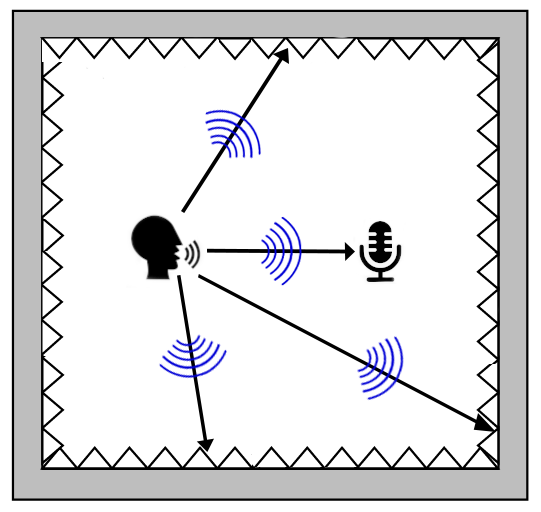
\includegraphics[scale=0.4]{camara_anecoica.png}
        \caption{Sala anecóica}
        \label{fig:Rooms_a}    
    \end{subfigure}
    \begin{subfigure}{.5\textwidth}
        \centering
        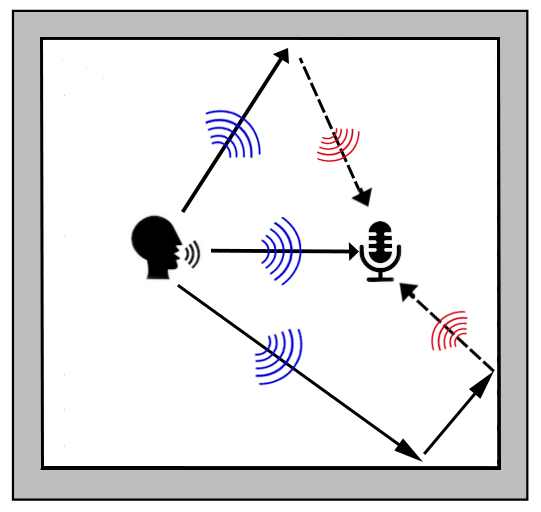
\includegraphics[scale=0.4]{camara_reverb.png}
        \caption{Sala reverberante}
        \label{fig:Rooms_b}    
    \end{subfigure}
    \caption{Representação de uma sala anecóica e reverberante.}
    \label{fig:Rooms}
\end{figure}

Observa-se na Figura \ref{fig:Rooms_a} uma representação de uma sala anecóica, onde o único áudio capturado pelo microfone é a onda sonora direta
enviada pela fonte, sem nenhuma reflexão do ambiente. Na sala reverberante, representada pela Figura \ref{fig:Rooms_b},
nota-se que o áudio capturado será uma combinação da onda sonora direta com as refletidas nas paredes. 
Este sinal reverberado pode ser modelado da seguinte forma:

\begin{equation} \label{eqn:model}
    y(t) = s(t) \ast h(t) + n(t)
\end{equation}

\noindent
onde $y(t)$ representa o sinal de voz em campo distante, $s(t)$ o sinal de voz anecóico, $h(t)$ a RIR e $n(t)$ o sinal de ruído que pode
estar presente no ambiente.
Dessa forma, é possível inferir que a RIR representa o modelo acústico de uma sala, para uma determinada combinação de fatores do ambiente, incluindo: 
temperatura e umidade relativa do ar, pressão atmosférica, material das paredes e posicionamento de móveis.
Reverberação causa degradação do sinal de voz, levando à perda de clareza na comunicação \cite{Speech_intellig_hear} e à redução de desempenho
de sistemas de reconhecimento de voz \cite{reverb_sup_speech_reg}. Este problema demonstra a necessidade de identificar dinamicamente o modelo acústico
do ambiente para que possam ser mitigadas as distorções nas amostras de voz gravadas e assim facilitar os algoritmos que usam esses sinais.

Este projeto é focado no estudo de uma forma de gerar RIRs simuladas a partir de RIRs reais devido à sua importância para diversas
aplicações usadas atualmente na indústria. Uma de suas aplicações é na análise e desenvolvimento de algoritmos de 
reconhecimento de voz robusta \cite{reverb_sup_speech_reg}, onde é necessário inferir a RIR para que possa ser feita a comparação entre
a supressão da reverberação ideal com a cega.
Outra aplicação da RIR é para desenvolvimento de algoritmos para localização e separação de fontes sonoras \cite{Source_sep_RIR},
onde as RIRs são usadas no auxílio do mapeamento acústico de ambientes reverberante através de algoritmos de separação de fonte às cegas.

\section{Desafios correlacionados à RIR}

É possível notar um recente aumento de pesquisas relacionadas à área de aprendizado de máquina no meio científico, especialmente no tópico de 
\textit{Deep Learning}) \cite{Study_SR_DL}. Observando a Figura \ref{fig:pub_DL} \cite{Jounal_Awareness_DL}, que apresenta quantidade de artigos
publicados por ano relacionados com Deep Learning, nota-se que após 2015, houve um aumento 
considerável de publicações em conferências do IEEE e em artigos e livros publicados pela editora Springer\textregistered.
Muitas dessas publicações são dedicadas para áreas de pesquisa relacionadas com áudio \cite{Study_SR_DL, Speech_proc_plus_DL, Source_Sep_DL}; de acordo com o artigo \cite{Survey_DL}, aproximadamente 20\% 
das publicações são voltadas para o tópico de reconhecimento de voz usando técnicas de \textit{Deep Learning} em suas metodologias.

\begin{figure} [H]
    \begin{subfigure}{1\textwidth}
        \centering
        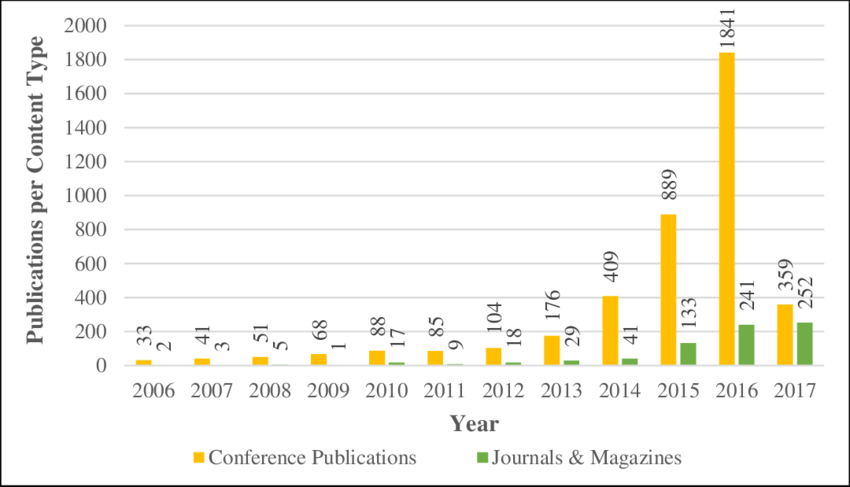
\includegraphics[scale=0.35]{pub_DL_IEEE.png}
        \caption{Publicações por ano - IEEE}    
    \end{subfigure}
    \begin{subfigure}{1\textwidth}
        \centering
        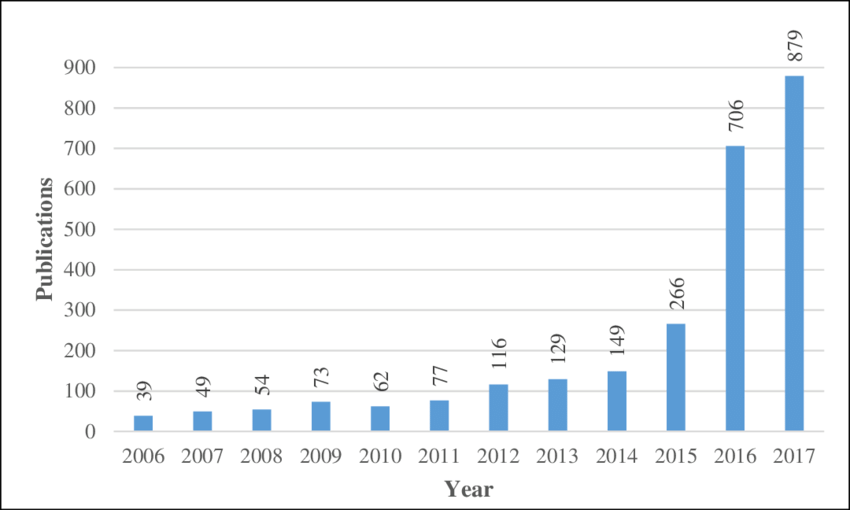
\includegraphics[scale=0.35]{pub_DL_Springer.png}
        \caption{Publicações por ano - Springer\textregistered}    
    \end{subfigure}
    \caption{Gráficos de quantidade de artigos publicados por ano relacionados com \textit{Deep Learning}.}
    \label{fig:pub_DL}
\end{figure}


Um dos maiores desafios enfrentados ao utilizar técnicas de \textit{Deep Learning} é de obter uma grande quantidade de dados para treinamento.
Podem ser observados exemplos em \cite{Estimation_RT_DRR,ACE_Data_Aug_Eval}, onde os autores necessitaram agrupar dados de mais de 5 bases contendo
RIRs para que fosse possível treinar e avaliar suas redes.
No caso de bases de dados que envolvem RIRs, o motivo de não existir uma alta variedade de dados é devido às dificuldades
de realizar gravações dos áudios \cite{Recording_RIR_2}.
A RIR pode ser obtida com diversos tipos de sinal de excitação: varreduras de seno, sequencias pseudo aletórias. 
De forma aproximada, pode-se usar estouro de balões \cite{Recording_RIR}.

%Para gerar um impulso sonoro, é necessário uma fonte sonora (por exemplo, um alto-falante) capaz de realizar uma varredura de senos com o mínimo de distorção
%possível, ou usar um equipamento para iniciar um som de decaimento rápido e de alta intensidade (por exemplo, um balão estourando) \cite{Recording_RIR}.
% A gravação do impulso requer microfones que estejam dentro de uma câmara anecóica, capacitando assim o microfone de gravar apenas o som vindo direto
% da fonte sonora, e não as ondas que são refletidas nas paredes.
Não menos importante, para aumentar a quantidade de amostras na base, deve-se gravar o áudio não só em diferentes posições no ambiente
e distâncias fonte-microfone, como também realizar estes mesmos procedimentos em ambientes diferentes, o que requer o transporte de diversos equipamentos
especializados entre localizações físicas.

\section{Aumento de Dados}

Aumento de Dados (AD) representa um conjunto de técnicas que são usadas em dados já existentes com o intuito de gerar versões
modificadas que aumentam a representatividade dos dados disponíveis para uma determinada aplicação. 
No contexto de \textit{Deep Learning}, essas técnicas tornam-se vitais para incrementar artificialmente bases de dados
para treinamento que não possuem uma alta variedade de amostras e isso inclui dados de áudio \cite{DL_Data_Aug_sc,Metric_Data_Aug_sc}.

\begin{figure} [H]
    \centering
    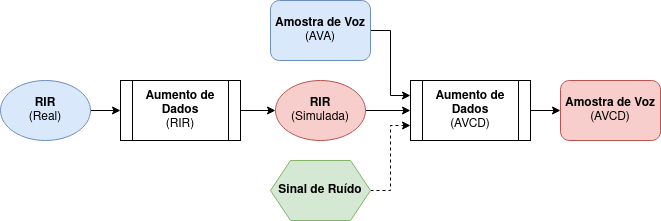
\includegraphics[scale=0.6]{flow-geral-ad.png}
    \caption{Fluxo geral de procedimentos para gerar sinais de voz reverberantes.}
    \label{fig:flow-geral}
\end{figure} 

No escopo deste trabalho, de acordo com a Figura \ref{fig:flow-geral} usaremos duas técnicas de aumento de dados para gerar amostras
de voz reverberantes. Uma das técnicas é voltada para simulação de RIRs, que altera suas propriedades para que possam ser simuladas diferentes condições
e posições em um determinado ambiente.

Outra técnica é desenvolvida para gerar amostras de voz em campo distante, usando as RIRs simuladas geradas pela primeira técnica e sinais de ruído.
Na segunda técnica, serão utilizados dois tipos de ruídos: pontual e de fundo.
O ruído pontual representa uma fonte sonora, além da amostra de voz anecóica, que está localizada no mesmo ambiente fechado em que ocorre 
a geração da AVCD, mas que não faz parte do sinal que se dejesa detectar. 
O ruído de fundo representa um fator sonoro externo ao ambiente fechado acrescentado à AVCD que prejudica a detecção da amostra de voz original em uma AVCD.

%Outra técnica é desenvolvida para simular ruídos no ambiente, que adiciona tanto ruídos pontuais em um trecho
%da amostra de voz, sendo este convoluído com a RIR real ou simulada, quanto um ruído de fundo. 
 


% ---------------------------------------------------------------
% Chapter 3 - Data Augmentation da Resposta ao Impulso do Ambiente
% ---------------------------------------------------------------
\chapter{Data Augmentation da Resposta ao Impulso do Ambiente}
\label{cap3}
Este capítulo é dedicado à implementação do primeiro algoritmo de \textit{Data Augmentation}, onde são geradas RIRs simuladas (RIRSM)
a partir de RIRs originais (RIRO), que foram gravadas em ambientes diversos e compõem o banco de dados AIR \cite{AIR_Database}. 
São observados os parâmetros de razão Direto-Reverberante (DRR) e tempo de reverberação (T60), que são
inferidos com base em uma RIRO e que serão manipulados pelo algoritmo para gerar RIRs que vão representar modelos acústicos diferentes.

\begin{figure} [H]
    \centering
    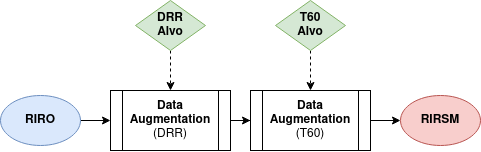
\includegraphics[scale=0.6]{flow-rir-aug.png}
    \caption{Fluxo de procedimentos para gerar a RIRSM.}
    \label{fig:flow-rir-aug}
\end{figure}

Este trabalho é uma implementação dos passos demonstrados no artigo \cite{RIR_Data_Aug}. A Figura \ref{fig:flow-rir-aug} especifica 
o fluxo de procedimentos implantados por este algoritmo, onde a DRR e T60 alvos são os valores escolhidos pelo usuário ou sorteados aleatoriamente,
que determinam as características da RIRSM. 

Antes de explicar os métodos usados, é necessário definir duas funções \cite{RIR_Data_Aug}:

\begin{align} 
    h_e(t) &= 
    \begin{cases} \label{eqn:rir-early}
        h(t), & t_d-t_0 \le t \le t_d+t_0 \\
        0, & \text{caso contrário,}
    \end{cases} \\
    h_l(t) &= 
    \begin{cases} \label{eqn:rir-late}
        h(t), & t < t_d - t_0 \\
        h(t), & t > t_d + t_0 \\
        0, & \text{caso contrário,}
    \end{cases}
\end{align}

\noindent
onde $t$ representa o tempo discreto, $t_d$ o tempo que as ondas sonoras diretas, ou seja, sem reflexão, levam da fonte até o destino de gravação,
$t_0$ a janela de tolerância, neste caso definida com o valor 2,5 ms \cite{RIR_Data_Aug}, 
$h(t)$ uma RIR, $h_e(t)$ as primeiras reflexões e $h_l(t)$ as reflexões tardias.
Neste algoritmo, $t_d$ é determinado da forma:

\begin{align} \label{eqn:t_d}
    %t_d = t_{max},\ onde \ \ h(t_{max}) = max(h(t))
    \begin{cases}
        t_d = t_{max},\\
        t_{max}, \ \text{onde} \ h(t_{max}) = max(|h(t)|)
    \end{cases}
    .
\end{align}


\section{Razão Direto-Reverberante (DRR)}


A DRR representa a razão entre a energia sonora da resposta ao impulso que atinge o alvo diretamente e a energia reverberante,
ou seja, que é refletida pelas paredes do ambiente fechado. Este parâmetro é calculado pela seguinte expressão:

\begin{equation} \label{eqn:DRR_def}
    DRR_{dB} = 10 \log_{10} \left( \frac{\sum_t h^2_e(t)}{\sum_t h^2_l(t)} \right).
\end{equation}

Para obter a $DRR_{dB}$ alvo desejada, aplica-se um fator de ganho escalar $\alpha$ na função das primeiras reflexões $h_e(t)$.
De acordo com \cite{RIR_Data_Aug}, para evitar descontinuidades durante o cálculo do fator $\alpha$, reescreve-se 
$h_e(t)$ em duas parcelas, uma que representa a janela direta no pico de intensidade de $h(t)$ e outra
que representa uma janela de resíduo de $h_e(t)$ formando, assim,

\begin{equation} \label{eqn:new-h_e}
    h'_e(t) = \alpha w_d(t) h_e(t) + [1 - w_d(t)]h_e(t),
\end{equation}

\noindent
onde $w_d(t)$ representa uma janela de Hann de duração de 5 ms, considerando-se uma janela de tolerância $t_0 = 2,5$ ms.
Substituindo na Equação (\ref{eqn:DRR_def}) $h_e(t)$ por $h'_e(t)$ e combinando com a Equação (\ref{eqn:new-h_e}), obtém-se
a seguinte equação quadrática;

\begin{equation} \label{eqn:DRR_quad_eqn}
    \begin{aligned} 
        \alpha^2 \sum_t w^2_d(t) h^2_e(t) +
        2 \alpha \sum_t [1 - w_d(t)] w_d(t) h^2_e(t) + \\
        \sum_t [1 - w_d(t)]^2 h^2_e(t) -
        10^{DRR_{dB}/10} \sum_t h^2_l(t)
        = 0 ,
    \end{aligned}
\end{equation}

O parâmetro $\alpha$ desejado será a raiz de maior valor. 
Uma ressalva deste procedimento é que se deve atentar para não escolher uma $DRR_{dB}$ que não seja muito menor que a original,
pois após a transformação de $h_e(t)$ para $h'_e(t)$, dependendo do valor de $\alpha$, é possível incidir em um caso onde
$max(h'_e(t)) < max(h_l(t))$, tornando a RIRSM impraticável.

A Figura \ref{fig:ir-early} exibe um exemplo de sinal $h(t)$ com o seu $h_e(t)$ após ser feita a modificação do DRR.
Comparando $h_e(t)$ com $h'_e(t)$, de acordo com a Figura \ref{fig:drr-da}, nota-se que $h'_e(t)$  está com uma intensidade 
maior, o que condiz a modificação do DRR de -4,5 dB para 4 dB neste exemplo.

\begin{figure}[H]
    \centering
    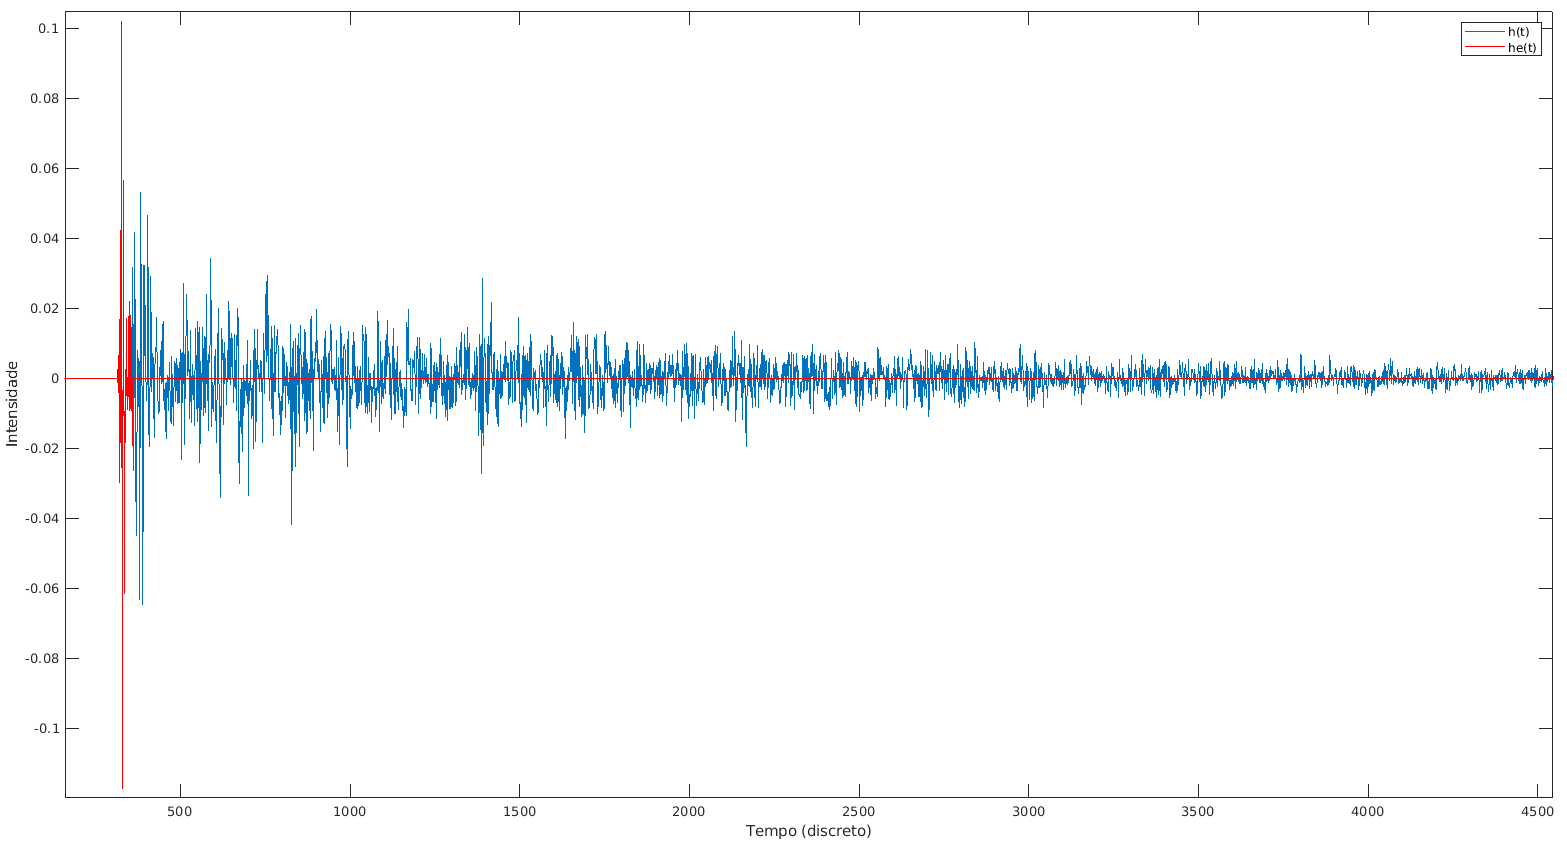
\includegraphics[scale=0.3]{ir-early.png}
    \caption{Um exemplo de $h(t)$ com $h_e(t)$, onde é feita a modificação do DRR de -4,5 para 4, marcado em vermelho.}
    \label{fig:ir-early}
\end{figure} 

\begin{figure}[H]
    \centering
    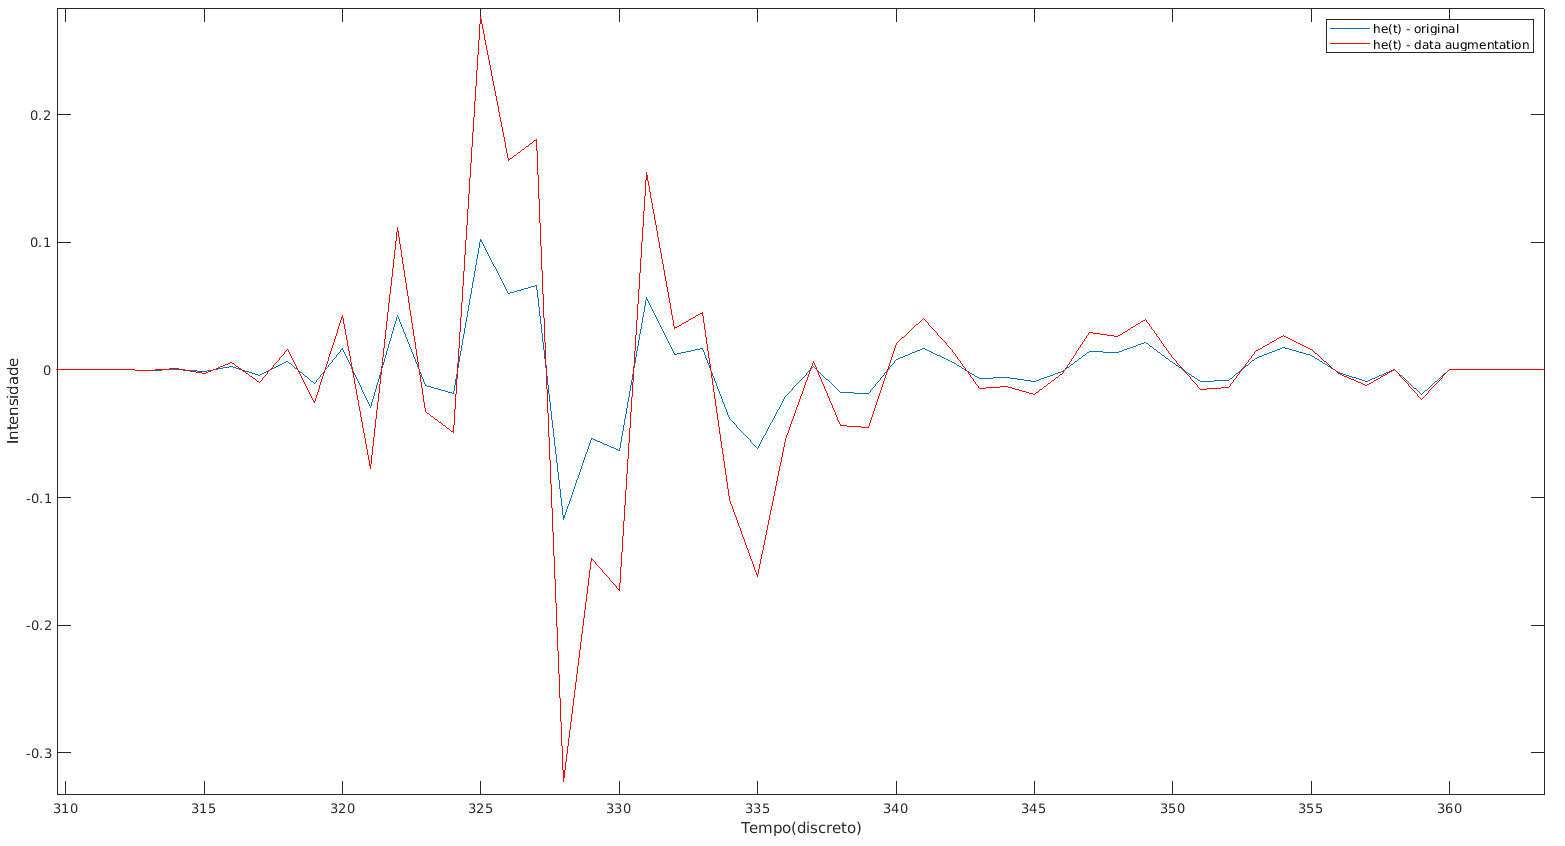
\includegraphics[scale=0.3]{drr-da.png}
    \caption{Um exemplo de $h_e(t)$ antes e depois da aplicação do algoritmo, original em azul ($DRR=-4,5$ dB) e o modificado em vermelho ($DRR=4$ dB).}
    \label{fig:drr-da}
\end{figure} 


\section{Tempo de Reverberação (T60)}


O T60, definido na equação \ref{eqn:T60-def}, representa a duração de tempo que leva para a energia sonora da RIR
no alvo decair 60 dB comparado à sua intensidade máxima. Geralmente, devido à dificuldade de se medir uma queda de 60 dB,
o parâmetro medido é o T20 ou o T30 e depois multiplica-se os seus valores por 3 e 2, respectivamente, para obter o T60,
assumindo-se um decaimento exponencial da envoltória da RIR.

\begin{align} \label{eqn:T60-def}
    \begin{cases}
        \text{T60} = t_f-t_i, \ \text{onde}\\
        t_i \rightarrow h(t_i) = max(h(t)) \\
        t_f \rightarrow 10 \log_{10} \left( h^2(t_i) - h^2(t_f) \right) = 60 \text{dB} \\
        %t_i, \ \text{onde} \ h(t_i) = max(h(t)) \\
        %t_f, \ \text{onde} \ 10 \log_{10} \left( h^2(t_i) - h^2(t_f) \right) = 60 \text{dB} \\
        %\text{T60} = t_f-t_i.
    \end{cases}
    .
\end{align}

Para realizar modificações na RIR, é necessário modelar a função das reflexões tardias. De acordo com \cite{RIR_Data_Aug},
um modelo normalmente usado é de um ruído gaussiano exponencialmente decadente, acrescido de um ruído residual, ou seja,

\begin{equation} \label{eqn:h_l-gauss}
    h_m(t) = A e^{-(t - t_o)/ \tau} n(t) u(t - t_o) + \sigma n(t)
    ,
\end{equation}

\noindent
onde $A$ representa o ganho da resposta ao impulso, $\tau$ a taxa de decaimento, $\sigma_m$ o desvio padrão do ruído residual, 
$n(t)$ um ruído gaussiano padrão (média nula e desvio padrão unitário), $t_o$ o valor temporal onde $h_l(t)$
tem o seu primeiro valor não nulo e $u(t)$ um degrau unitário.
Neste trabalho, diferente da implementação do algoritmo em \cite{RIR_Data_Aug}, é considerada apenas a taxa de decaimento
do espectro de frequência por completo da RIR, ao invés de dividi-la em subbandas e analisar 
a taxa de decaimento para cada faixa de frequência.

Os parâmetros $A$, $\tau$ e $\sigma$ são estimados de acordo com o padrão definido na ISO 3382-1 \cite{ISO-3382}.
Seja $T60_d$ o valor de T60 alvo para DA, é possível inferir a taxa de decaimento através da equação

\begin{equation} \label{eqn:decay-rate-t60}
    T60_d = \ln(1000) \tau_d T_s
    ,
\end{equation}

\noindent
onde $\tau_d$ representa a taxa de decaimento alvo e $T_s$ o intervalo de amostragem.
A DA do tempo de reverberação é feita multiplicando-se $h_l(t)$ pela exponencial

\begin{equation} \label{eqn:DA-T60}
    h'_l(t) = h_l(t) e^{-(t - t_o) \frac{\tau - \tau_d}{ \tau \tau_d} }
    .
\end{equation}

Por fim, a RIRSM completa, $h'(t)$, pode ser representada pela equação

\begin{equation} \label{eqn:RIRSM}
    h'(t) = h'_e(t) + h'_l(t)
    .
\end{equation}

A Figura \ref{fig:ir-late} exibe um exemplo de sinal $h(t)$ com o seu $h_l(t)$ após ser feita a modificação do T60.
Comparando $h_l(t)$ com $h'_l(t)$, de acordo com a Figura \ref{fig:t60-da}, nota-se que $h'_l(t)$  está com uma intensidade 
maior, o que condiz a modificação do T60 de 1,38 para 2,6 segundos neste exemplo.

\begin{figure}[H]
    \centering
    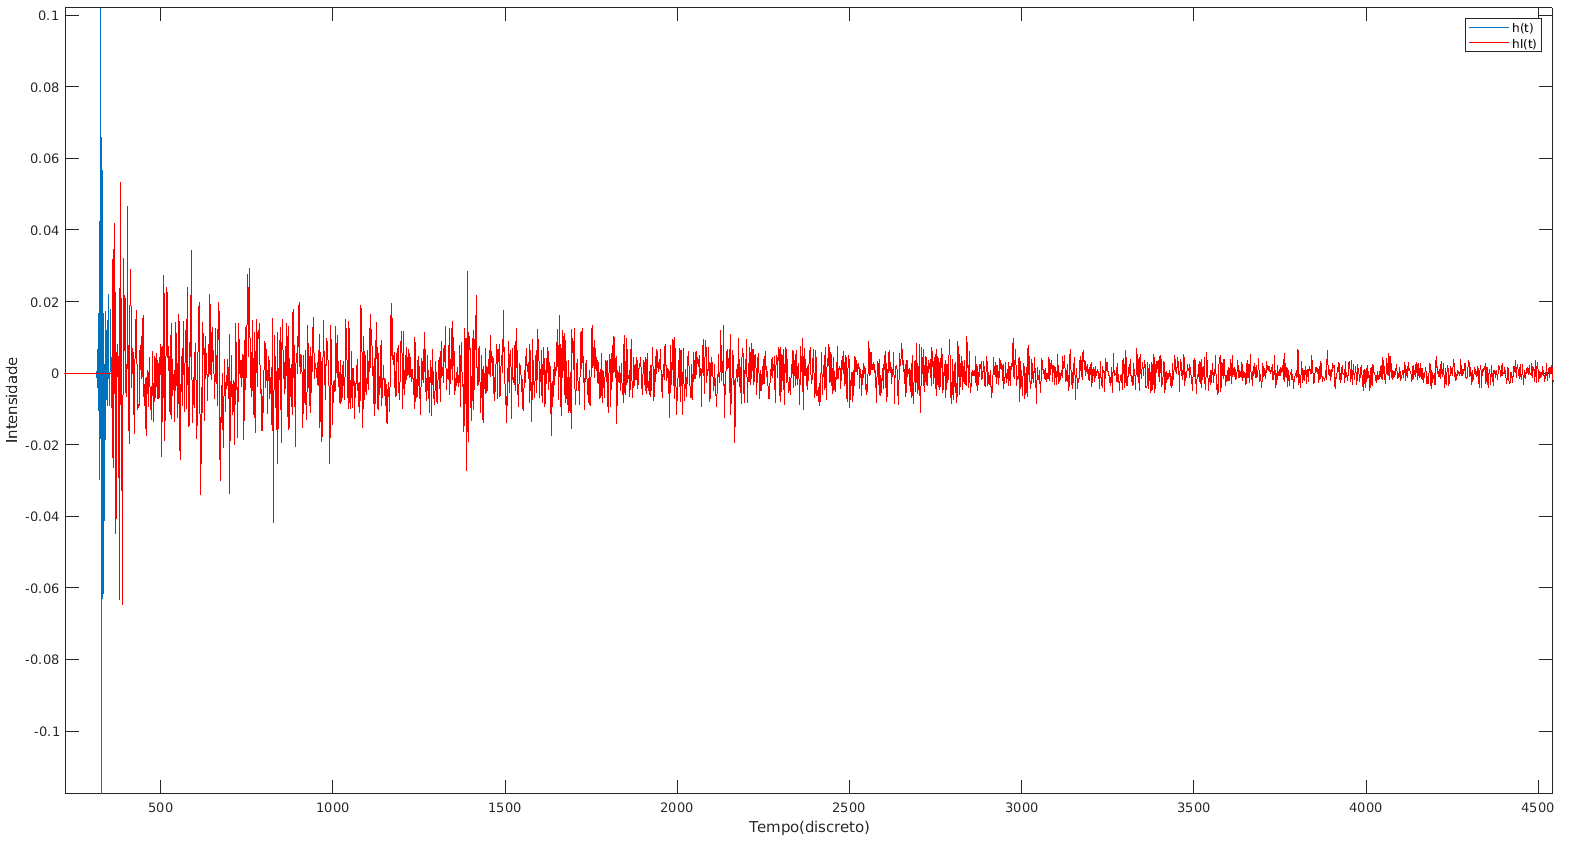
\includegraphics[scale=0.3]{ir-late.png}
    \caption{Um exemplo de $h(t)$ com $h_l(t)$, onde é feita a modificação do T60 de 1,38 para 2,6 segundos, marcado em vermelho.}
    \label{fig:ir-late}
\end{figure} 

\begin{figure}[H]
    \centering
    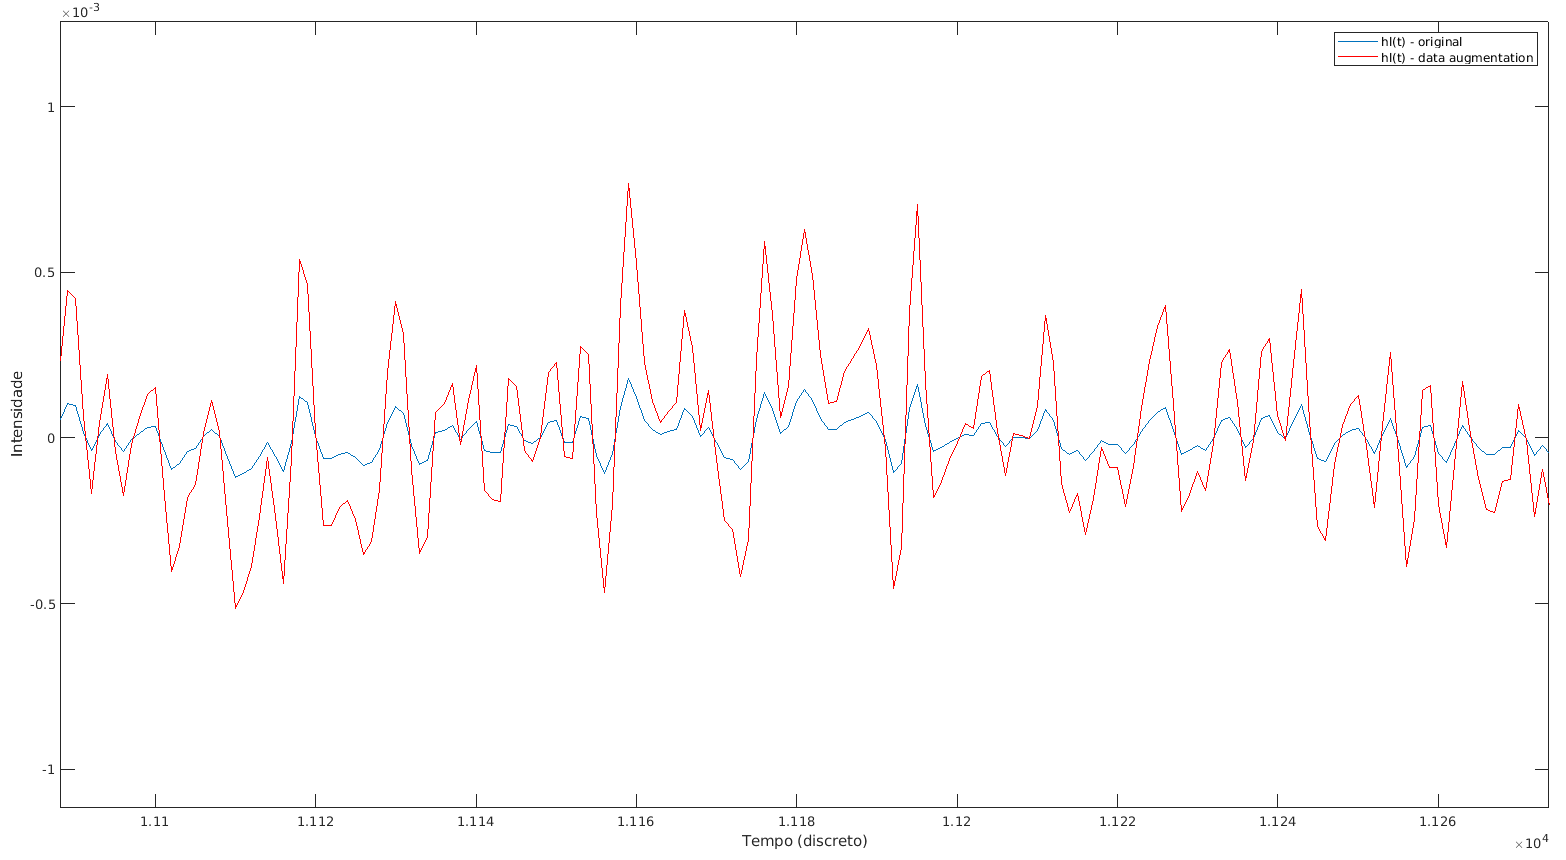
\includegraphics[scale=0.3]{t60-da.png}
    \caption{Um exemplo de um trecho ao final de $h_l(t)$ antes e depois da aplicação do algoritmo, original em azul ($T60=1,38$ s) e o modificado em vermelho ($T60=2,6$ s).}
    \label{fig:t60-da}
\end{figure} 

% ---------------------------------------------------------------
% Chapter 4 - Desenvolvimento de Sinais de Voz Reverberadas Simuladas com Ruídos
% ---------------------------------------------------------------
\chapter{Desenvolvimento de Sinais de Voz Reverberadas Simuladas com Ruídos}
\label{cap4}
Este capítulo é dedicado ao desenvolvimento do segundo algoritmo de \textit{Data Augmentation}, onde são geradas as amostras de voz 
reverberadas em campo-distante (AVCDs) usando: amostras de voz anecóicas (AVAs), RIRSM, sinais de ruído pontuais (SRPs) e de fundo (SRFs).

\begin{figure} [H]
    \centering
    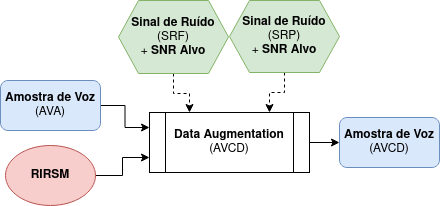
\includegraphics[scale=0.65]{flow-voz-aug.png}
    \caption{Fluxo de procedimentos para gerar a AVCD.} 
    \label{fig:flow-voz-rev}
\end{figure}

Este trabalho é uma implementação dos passos demonstrados no artigo \cite{Speech_Rec}. A figura \ref{fig:flow-voz-rev} especifica 
o fluxo de procedimentos implantados por este algoritmo, onde o SRP, SRF e SNR alvos são aleatoriamente escolhidos, 
dentro de uma base de dados de ruídos e uma faixa de valores definidas pelo usuário, que determinam as características da AVCD. 

\section{Simulação de fala em campo distante} 

Sinais de voz em campo-distante são tipicamente compostos por uma combinação de VR, SRP (assumindo que a fonte do ruído pontual encontra-se 
no mesmo ambiente da VR) e SRF (assumindo que não é afetado pelo modelo acústico do ambiente).
É possível modelar uma AVCD conforme a equação

\begin{equation} \label{eqn:AVCD-model}
    S_{cd}[t] = S_a[t] \ast h[t] + \sum_i n_{pi}[t] \ast h[t] + n_f[t]
    ,
\end{equation}

onde $S_{cd}[t]$ representa a AVCD, $S_a[t]$ a AVA, $h[t]$ a RIR, $n_{pi}[t]$ o i-ésimo SRP e $n_f[t]$ o SRF.
Neste trabalho, diferente da implementação do algoritmo em \cite{Speech_Rec}, é considerado apenas uma única RIR
para gerar a AVCD, ou seja, os ruídos pontuais são convoluídos com a mesma RIR que é usada para a fonte de voz.


Abaixo segue o algoritmo que é usado para gerar sinais de voz em campo-distante simuladas. 
\bigbreak
\bigbreak

\begin{algorithm} [H] 
    \caption{Procedimentos para gerar AVCD}
    \label{alg:AVCD-gen}

    \KwIn{$fl_p$ : Flag de inclusão de ruído pontual} 
    \KwIn{$fl_g$ : Flag de inclusão de ruído de fundo} 
    \KwIn{$m$ : Quantidade de ruídos pontuais} 
    \KwIn{$SNR_{up}$ : Limite superior de SNR} 
    \KwIn{$SNR_{dw}$ : Limite inferior de SNR} 

    $S_r[t] \gets S_a[t] \ast h[t]$ : Convolução da RIR com AVA

    \If{$fl_p = true$}
    {
        \For{$i = 1$ até $m$}
        {
            Escolha aleatória de um ruído pontual $n_{pi}[t]$ da biblioteca de ruído. \\
            Escolha aleatória de uma SNR Alvo $SNR_t$ compreendida dentro do intervalo $[SNR_{dw},SNR_{up}]$. \\
            Dedução do fator $\alpha$ a partir da $SNR_t$ para corrigir a intensidade de $n_{pi}[t]$. \\
            Escolha aleatória de offset $o_t$ compreendida dentro do intervalo $(0,\text{duração(t)})$. \\
            $S_r[t] \gets S_r[t] + \alpha \text{offset}(n_{pi}[t] \ast h[t], o_t)$ : Adição de SRP na AVR.
        }
    }
    \If{$fl_g = true$}
    {
        Escolha aleatória de um ruído de fundo $n_f[t]$ da biblioteca de ruído. \\
        Escolha aleatória de uma SNR Alvo $SNR_t$ compreendida dentro do intervalo $[SNR_{dw},SNR_{up}]$. \\
        Dedução do fator $\alpha$ a partir da $SNR_t$ para corrigir a intensidade de $n_f[t]$. \\
        Estender ou encurtar $n_f[t]$ até que $\text{duração}(n_f[t]) = \text{duração}(S_r[t])$
        $S_r[t] \gets S_r[t] + \alpha n_f[t]$ : Adição de SRF na AVR.
    }

\end{algorithm}
%\bigbreak
%\bigbreak
\pagebreak


Neste trabalho, o algoritmo de geração de AVCD usa as RIRSM geradas através do primeiro algoritmo, diferente do que foi implantado
em \cite{Speech_Rec}, onde foram geradas RIRs de forma completamente digital \cite{RIR_sim_image}, ou seja, sem usar RIRs reais 
como base para \textit{Data Augmentation}.
Nota-se também que o algoritmo permite habilitar ou não o uso de cada tipo de ruído para que possa aumentar a variedade de dados gerados, além
de acomodar mais propósitos de treinamentos de \textit{Deep Learning}.


\begin{figure} [H]
    \centering
    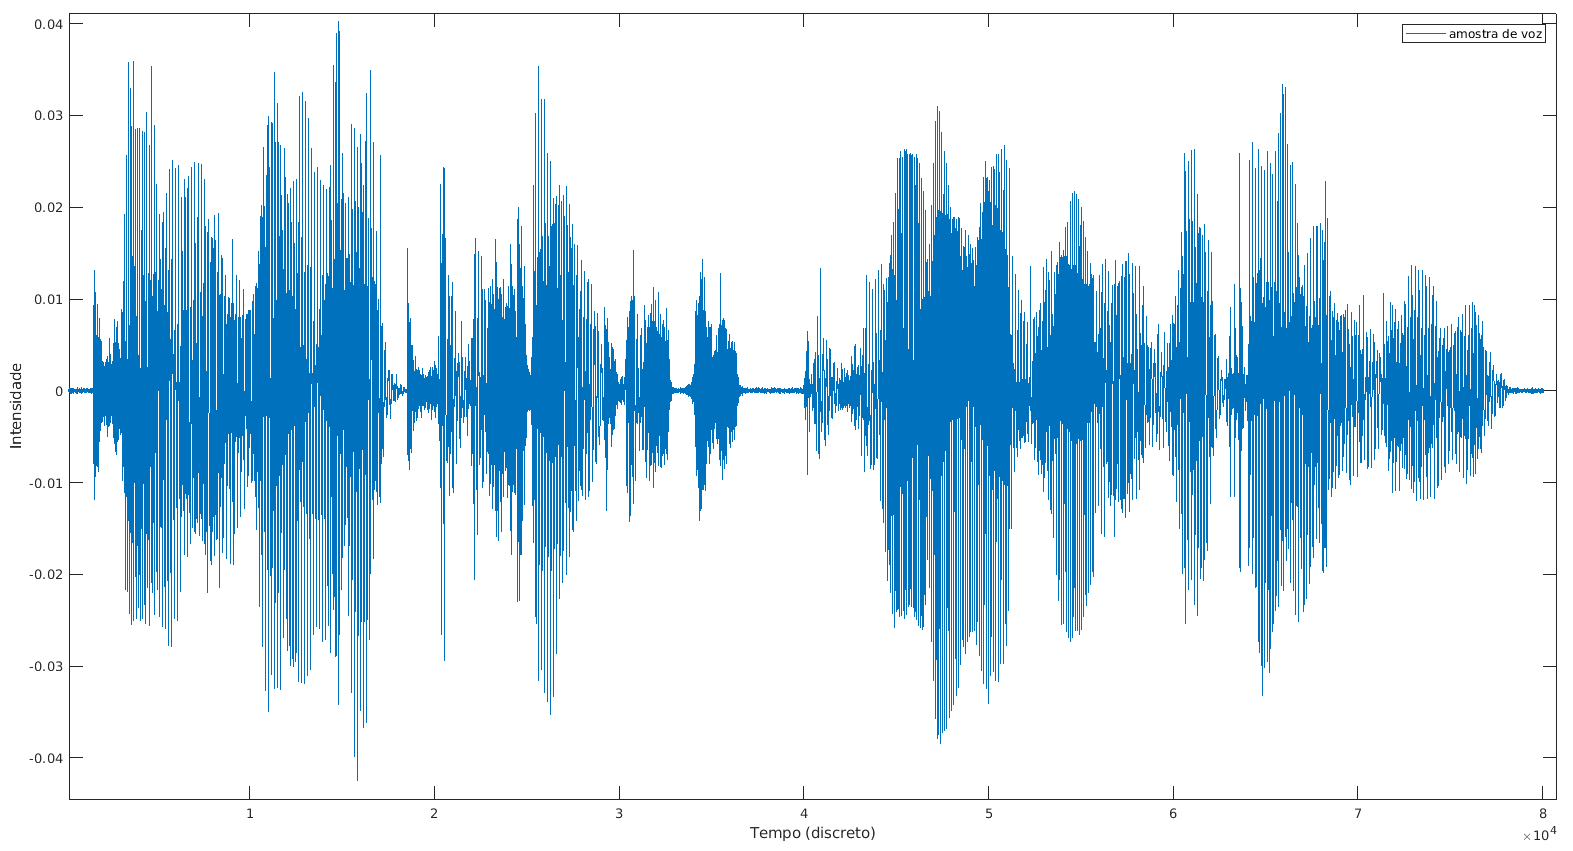
\includegraphics[scale=0.3]{voice-sample.png}
    \caption{Exemplo de amostra de voz anecóica.}
    \label{fig:voice-sample}
\end{figure} 

\begin{figure} [H]
    \centering
    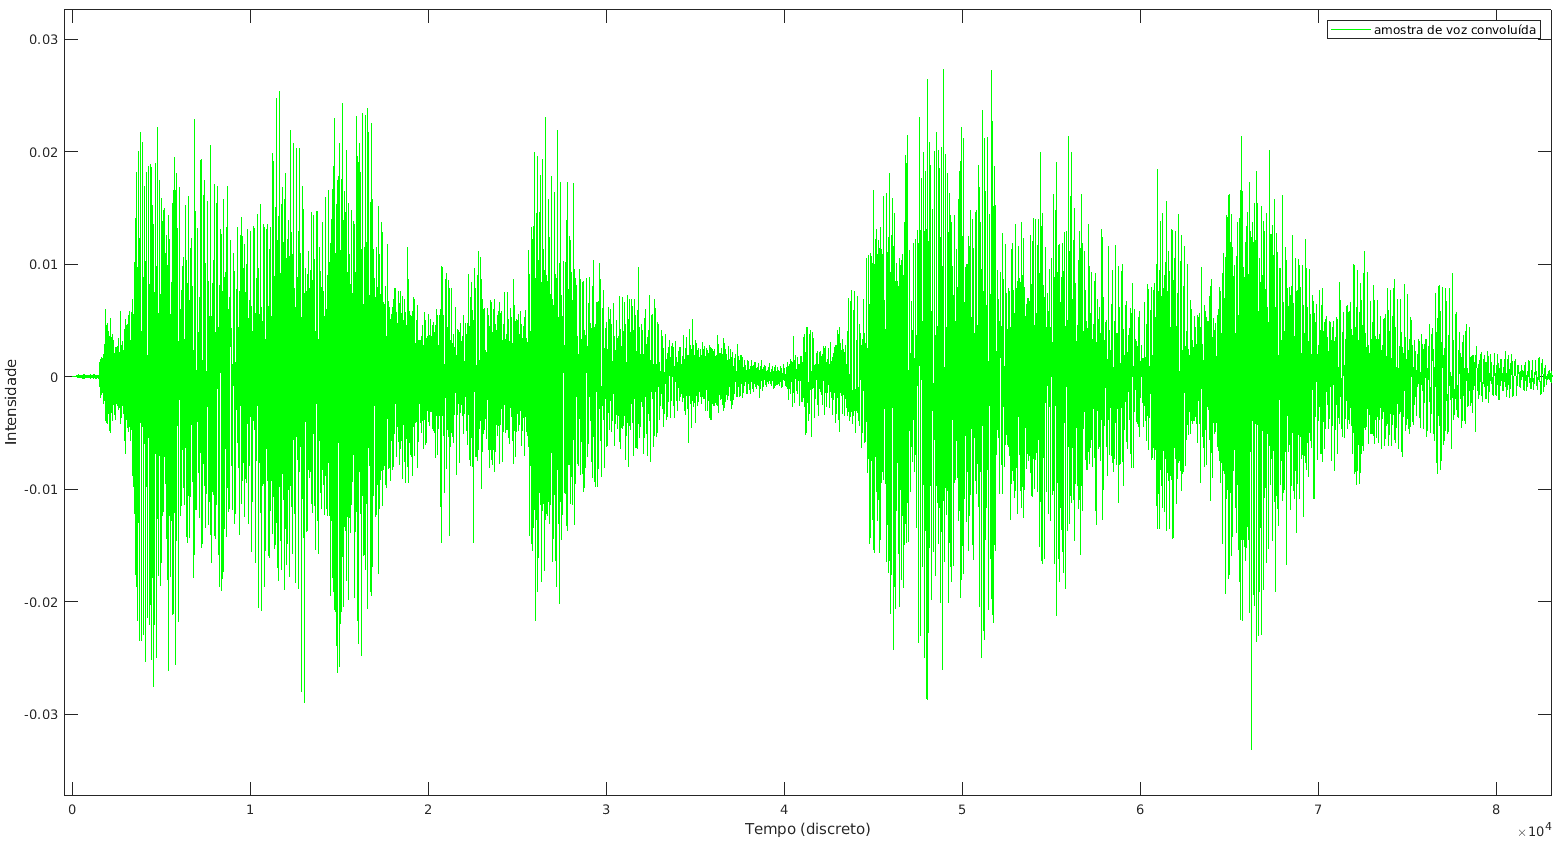
\includegraphics[scale=0.3]{voice-aug.png}
    \caption{Exemplo de amostra de voz reverberante, convoluída com uma RIRSM.}
    \label{fig:voice-aug}
\end{figure} 

\begin{figure} [H]
    \centering
    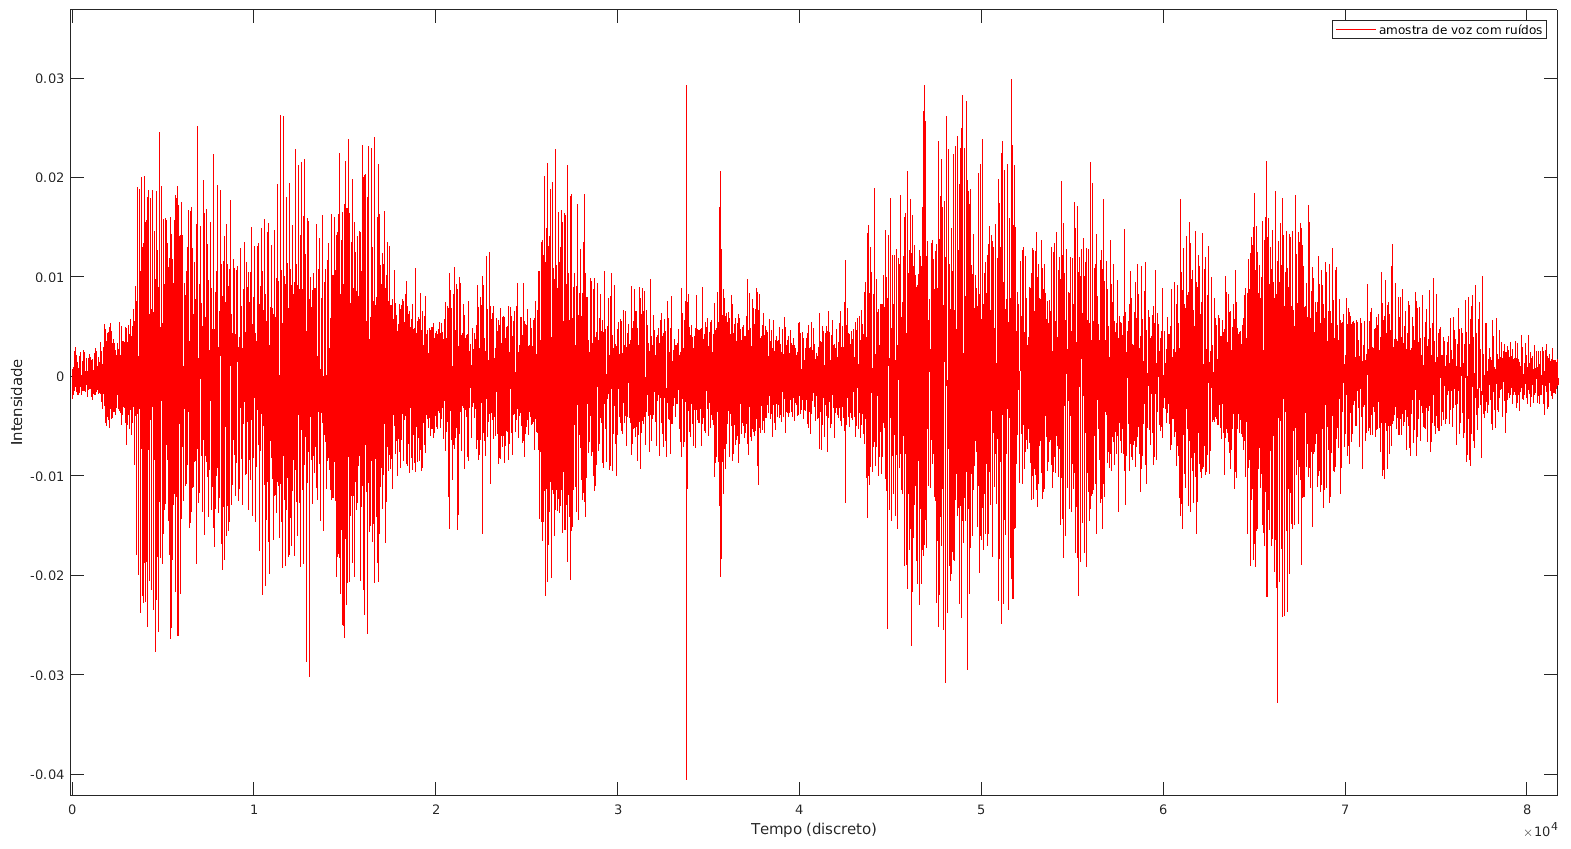
\includegraphics[scale=0.3]{voice-noise.png}
    \caption{Exemplo de amostra de voz em campo distante, representado pela voz reverberada mais os ruídos adicionados pelo segundo método de DA.}
    \label{fig:voice-noise}
\end{figure} 

% ---------------------------------------------------------------
% Chapter 5 - Resultados Experimentais
% ---------------------------------------------------------------
\chapter{Resultados Experimentais}
\label{cap5}
Este capítulo apresenta as bases de dados que serão usadas para gerar os resultados experimentais.
Para a aplicação da metodologia deste trabalho, é necessário três fontes de dados:

\begin{itemize}
    \item base de dados com amostras de voz anecoicas para convolução com as RIRSMs,
    \item base de dados com RIRs reais para o primeiro nível de \textit{Data Augmentation}, gerando as RIRSMs,
    \item base de dados com SRPs e SRFs para o segundo nível de \textit{Data Augmentation}, gerando as AVCDs.
\end{itemize}


\section{Base de amostras de voz anecoicas}

A base de AVAs usada consiste na leitura de textos em inglês por 4 pessoas diferentes (duas vozes masculinas e duas femininas).
Os arquivos de áudio são disponibilizados em formato WAV, com frequência de amostragem de 16 KHz, e cada gravação tem duração
em torno de 5 a 6 segundos; no caso deste trabalho, foram concatenadas duas frases por pessoa na mesma 
gravação devido ao tempo de duração dos ruídos pontuais que serão adicionados para a geração de AVCDs.

A tabela \ref{tbl:voice} descreve as gravações usadas neste projeto.

\begin{table} [H]
    \centering
    \caption{Descrição dos textos pronunciados por locutor.}
    \label{tbl:voice}
    \begin{tabularx}{\textwidth}{l|c|p{9cm}} 
        
        \multicolumn{1}{c|}{\textbf{Nome}} & \multicolumn{1}{|c|}{\textbf{Código}} & \multicolumn{1}{|c}{\textbf{Texto}} \\
        %\textbf{Nome} & \textbf{Código} & \textbf{Texto} \\
        \hline 

        Homen 1 - Texto 1 & H1-T1 & \textit{This food is too spicy he complained. Young man can be very arrogant and rude.} \\
        Homen 1 - Texto 2 & H1-T2 & \textit{So Marcus owned a big shipping company. Their eyes met across the table.} \\
        Homen 2 - Texto 1 & H2-T1 & \textit{Time is running out for the scientists. If you knew Julie like I know Julie.} \\
        Homen 2 - Texto 2 & H2-T2 & \textit{Your new dress is breathtaking darling. Her first book was published last year.} \\
        Mulher 1 - Texto 1 & M1-T1 & \textit{Among them are canvases from a young artist. Building from the ground up is very costly.} \\
        Mulher 1 - Texto 2 & M1-T2 & \textit{Next year we will see several more exibitions. The number of works on view will increase.} \\
        Mulher 2 - Texto 1 & M2-T1 & \textit{An enourmous quake rocked the island. Eventually he hopes to solve all the problems.} \\
        Mulher 2 - Texto 2 & M2-T2 & \textit{Eventually he hopes to solve all the problems. Faulty installation can be blamed for this.} \\
        
    \end{tabularx}
\end{table}

\section{Base de RIRs - Aachen Impulse Response database (AIR)}

A base de AIR \cite{AIR_Database} é um conjunto de respostas ao impulso sonoras que foram medidas em diversas salas.
O objetivo dessa base é de fornecer dados para estudos de algoritmos de processamento de sinais para ambientes reverberados.

Ela é composta primariamente por RIRs binaurais medidas com ou sem uma cabeça falsa de manequim em locais com diferentes
propriedades acústicas; é importante frisar também que a base possui gravações com diferentes distâncias entre a fonte sonora
e os microfones para a mesma sala, gerando outros tempos de reverberação.
A base também possui gravações em diferentes ângulos azimutais com o objetivo de auxiliar algoritmos de detecção
de direção da fonte sonora; para o escopo deste projeto, tais RIRs não serão usadas. 

\begin{table} [H]
    \centering
    \caption{Configurações de RIRs disponíveis na AIR.}
    \label{tbl:rir}
    \begin{tabularx}{\textwidth}{l|c|c|c|l}
        
        \multicolumn{1}{c|}{\textbf{Sala}} & \multicolumn{1}{c|}{\textbf{Descrição}} & \multicolumn{1}{|c|}{\textbf{Canais}} &
        \multicolumn{1}{|c|}{\textbf{Cabeça}} & \multicolumn{1}{c}{\textbf{Distâncias}} \\
        %\textbf{Sala} & \textbf{Descrição} & \textbf{Canais} & \textbf{Cabeça} & \textbf{Distâncias (m)} \\
        \hline 

        Booth & cabine de estúdio & E/D & S/N & 0,5/1/1,5 \\
        Office & escritório comercial & E/D & S/N & 1/2/3 \\
        Meeting & sala de reuniões & E/D & S/N & 1,45/1,7/1,9/2,25/2,8 \\
        Lecture & sala de aula & E/D & S/N & 2,25/4/5,56/7,1/8,68/10,2 \\
        Stairway & escadaria aberta & E/D & S/N & 1/2/3 \\
        Aula Carolina & igreja de área 570m² & E/D & S/N & 1/2/3/5/15/20 

    \end{tabularx}
\end{table}

Os ambientes em que foram feitas as gravações de RIRs e suas respectivas configurações são definidos na tabela \ref{tbl:rir}.
Todos os ambientes usados possuem gravações com ambos os canais esquerdo e direito (E/D) e com configuração com ou sem a cabeça
falsa. As RIRs foram salvas como vetores binários de precisão dupla de ponto flutuante (formato MAT, que pode ser importado
via MATLAB\textregistered).

\section{Base de ruídos - MUSAN}

A base de MUSAN (\textit{A Music, Speech, and Noise Corpus}) \cite{noiseLib} consiste em um conjunto de músicas de diversos gêneros,
amostras de voz de doze línguas e uma variedade de ruídos técnicos e não-técnicos.
Ela foi criada primariamente para auxiliar no treinamento de modelos voltados para detecção de atividade de voz, contudo ela 
é usada também para teste de algoritmos processamento de sinais na área de áudio, por exemplo, reconhecimento de voz e orador.
Uma das vantagens dessa base é o fato dela ser uma compilação de áudios com fontes em domínios públicos, facilitando a 
distribuição dos áudios para uso da comunidade científica.

No escopo deste projeto, será usado somente a seção de ruídos da base, composta por seis horas de áudio no total.
A seção de ruídos é composta por sons técnicos de curta duração, que são usados como SRPs no segundo processo de 
\textit{Data Augmentation}, e por sons de ambiente, usados como SRFs no mesmo processo.

\begin{table} [H]
    \centering
    \caption{Descrição dos tipos de ruídos pontuais usados da base MUSAN.}
    \label{tbl:noise}
    \begin{tabular}{c|l}

        \multicolumn{1}{c|}{\textbf{Código}} & \multicolumn{1}{c}{\textbf{Descrição}} \\
        %\textbf{Código} & \textbf{Descrição} \\
        \hline 

        RP-1 & miado de gato \\
        RP-2 & madeira sendo lixada \\
        RP-3 & buzina de automóvel \\
        RP-4 & porta abrindo \\
        RP-5 & grampeador \\
        RP-6 & teclado de forno de microondas \\
        RP-7 & \textit{zipper} sendo fechado \\
        RP-8 & latido de cão \\
        RP-9 & batendo em uma porta \\
        RP-10 & espirro \\
        RP-11 & campainha \\
        RP-12 & vibrador de celular \\

    \end{tabular}
\end{table}

\begin{table} [H]
    \centering
    \caption{Descrição dos tipos de ruídos de fundo usados da base MUSAN.}
    \label{tbl:noise-bg}
    \begin{tabular}{c|l}

        \multicolumn{1}{c|}{\textbf{Código}} & \multicolumn{1}{c}{\textbf{Descrição}} \\
        %\textbf{Código} & \textbf{Descrição} \\
        \hline 

        RF-1 & avião decolando em aeroporto \\
        RF-2 & sala de máquinas \\
        RF-3 & estática \\
        RF-4 & sons de floresta \\

    \end{tabular}
\end{table}

As tabelas \ref{tbl:noise} e \ref{tbl:noise-bg} indicam os ruídos separados da base para gerar AVCDs.
Os arquivos de áudio são disponibilizados em formato WAV, com frequência de amostragem de 16 KHz. 

% ---------------------------------------------------------------
% Chapter 6 - Conclusões
% ---------------------------------------------------------------
\chapter{Conclusões}
\label{cap6}
\paragraph{}Tratam-se das considerações finais do trabalho, mostrando que os objetivos foram cumpridos e enfatizando as descobertas feitas durante o projeto. Em geral reserva-se um ou dois parágrafos para sugerir trabalhos futuros.

\paragraph{}Observe que neste modelo a conclusão é numerada pelo numeral 3, mas o projeto não tem a obrigatoriedade de possuir apenas 3 capítulos. Alias, espera-se que tenha mais que isso.



% ---------------------------------------------------------------
% Bibliografia
% ---------------------------------------------------------------
\normalsize
\cleardoublepage
\addcontentsline{toc}{chapter}{Bibliografia}
\bibliographystyle{coppe}
\bibliography{biblio}

% ---------------------------------------------------------------
% Apêndices 
% ---------------------------------------------------------------
   \appendix
   % ---------------------------------------------------------------
   % Apêndice A
   % ---------------------------------------------------------------
   \chapter{O que é um apêndice?}
   \label{ApendiceA}
   texto
   % ---------------------------------------------------------------
   % Apêndice B
   % ---------------------------------------------------------------
   \chapter{Encadernação do Projeto de Graduação}
   \label{ApendiceB}
   O código fonte da implementação da metodologia deste trabalho está disponível no \textit{GitHub}.
Segue o link abaixo.

https://github.com/afonsobm/RIR-Augmentation-MATLAB
   % ---------------------------------------------------------------
   % Apêndice C
   % ---------------------------------------------------------------
   \chapter{O que é um anexo?}
   \label{ApendiceC}
   \paragraph{}Documentação não elaborada pelo autor, ou elaborada pelo autor mas constituindo parte de outro projeto.   

\backmatter

\end{document}
